\chapter{Internet of Things}

The term Internet of Things (IoT) was first coined by Kevin Ashton in 1999. It refers to the concept of connecting various devices to the Internet and enabling them to communicate and exchange data. The IoT ecosystem consists of three main components: sensors, connectivity, and cloud computing. Sensors are responsible for collecting data from the physical world, connectivity enables the transmission of data to the cloud, and cloud computing provides the necessary infrastructure for data storage and processing \cite{ibm-iot}, \cite{javapoint-iot}, \cite{Capra2019EdgeWorld}.
The IoT ecosystem is illustrated in Figure \ref{fig:iot-ecosys}.
\begin{figure}[h!]
    \centering
    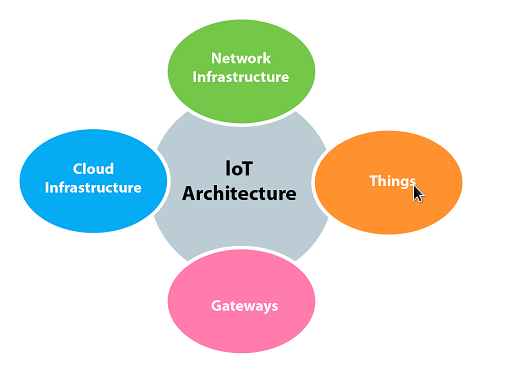
\includegraphics[width=0.8\textwidth]{pict/iot-ecosys.png}
    \caption{IoT Ecosystem \cite{javapoint-iot}}
    \label{fig:iot-ecosys}
\end{figure}

\section*{Examples of IoT applications}
Some of the most prominent examples of the applications of IoT include smart cities, smart homes, smart grids, and smart agriculture. The general principle of the workings of these IoT applications is illustrated in Fig:\ref{fig:iot-architecture}.

\begin{figure}[h!]
    \centering
    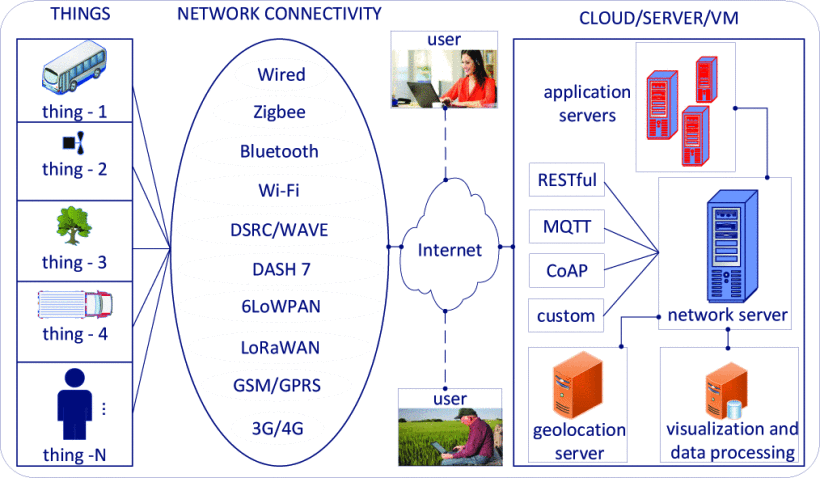
\includegraphics[width=0.98\textwidth]{pict/iot-architecture.png}
    \caption{Network architecture of IoT and applications \cite{iot-overview}}
    \label{fig:iot-architecture}
\end{figure}

\subsection*{Smart Cities}
The concept of smart cities aims to improve the quality of life by utilizing IoT technology to enhance the efficiency of urban services. Smart cities can be achieved by implementing IoT solutions in various areas such as transportation and energy. For example, smart parking systems can help drivers find available parking spots, thus reducing traffic congestion and air pollution. Smart street lighting can automatically adjust the brightness of street lights based on the time of day, weather conditions, and traffic density. Smart waste management systems can optimize the collection of garbage by monitoring the
filling level of waste bins \cite{ibm-iot}, \cite{javapoint-iot}, \cite{iot-overview}.

\subsection*{Smart Homes} 
similar to smart cities, in homes, smart home devices can be controlled remotely using a smartphone or a voice assistant. For example, smart thermostats can automatically adjust the temperature based on the time of day and weather conditions. Smart lighting systems can automatically turn on and off based on the presence of people in the room. Smart security systems can monitor the surroundings and alert the homeowner in case of suspicious activity \cite{javapoint-iot}, \cite{iot-overview}. 

\subsection*{Smart Grids}
Smart grids are electrical grids that utilize IoT technology to improve the efficiency of energy distribution. For example, smart meters can monitor the consumption of electricity and provide real-time data to utility companies. Smart meters can also enable dynamic pricing, which allows consumers to save money by using electricity during off-peak hours. Smart grids can also improve the reliability of energy distribution by automatically detecting faults in the grid \cite{javapoint-iot}, \cite{iot-overview}. 

\subsection*{Smart Agriculture}
Smart agriculture is another example of IoT applications that aim to improve the efficiency of agricultural production. For example, smart sensors can monitor the soil moisture level and provide real-time data to farmers. Smart sensors can also enable irrigation management, which allows farmers to save water by
automatically adjusting the irrigation schedule based on the weather conditions. Smart agriculture can also improve the efficiency of livestock production by enabling livestock monitoring, which allows farmers to monitor the health status of their animals remotely \cite{ibm-iot}, \cite{javapoint-iot}.

\section{LPWAN Technologies}
Low Power Wide Area Network (LPWAN) technologies are designed specifically for IoT applications that require long-range communication and low power consumption and also machine to machine (M2M) communication applications. LPWAN technologies can be classified into two categories: cellular and non-cellular. Cellular LPWAN technologies include NB-IoT, LTE Cat-M, and EC-GSM-IoT.
Non-cellular LPWAN technologies include Sigfox and LoRaWAN. In this section, we will discuss the characteristics of these technologies and compare them with each other based on their performance metrics such as data rate, range, and power consumption \cite{LPWAN-Considerations}, \cite{LPWAN-overview}.

\begin{figure}[h!]
    \centering
    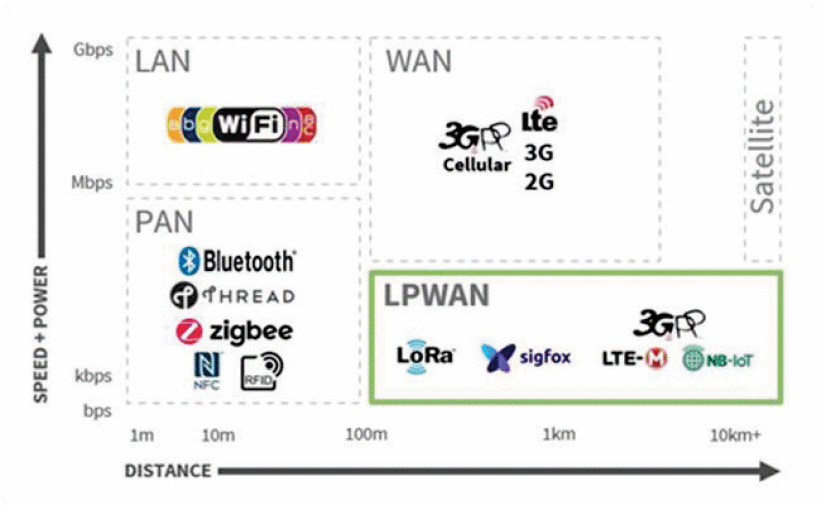
\includegraphics[width=0.98\textwidth]{pict/lpwan.png}
    \caption{Range of different Wireless Technologies and LPWAN \cite{LPWAN-overview}}
    \label{fig:lpwan-overview}
\end{figure}

\subsection{NB-IoT} 
Narrowband Internet of Things (NB-IoT) is a cellular LPWAN technology that was standardized by \href{https://www.3gpp.org/news-events/3gpp-news/nb-iot-complete}{3GPP} in Release 13 in 2016 \cite{ubox_nb-iot}, \cite{NB_IoT-rohde}, \cite{Rastogi2020NarrowbandStudy}, \cite{Wang2017AThings}, \cite{Kellerman}. In Czech Republic, Vodafone was the first
operator to launch NB-IoT network in 2017 \cite{vodafone-iot}. 

NB-IoT operates in the licensed spectrum and can coexist with other cellular technologies such as LTE and GSM. NB-IoT supports three deployment modes: in-band, guard-band, and standalone. In-band mode uses the same carrier frequency as LTE, while guard-band mode uses the guard band between LTE carriers. Standalone mode
uses a dedicated carrier frequency for NB-IoT \cite{NB_IoT-rohde}, \cite{ericsson-tech-review}. 

The \href{https://www.3gpp.org/news-events/3gpp-news/nb-iot-complete}{3GPP} defines 3 power classes for NB-IoT i.e: Class 3(23 dBm), Class 5 (20 dBm) and Class 6 (14dBm) \cite{NB_IoT-rohde}.

NB-IoT provides the following features \cite{ubox_nb-iot}, \cite{NB_IoT-rohde}, \cite{ericsson-tech-review}
\begin{itemize}
    \item very low power consumption
    \item excellent extended range in buildings and underground
    \item easy deployment into existing cellular network architecture
    \item network security and reliability
    \item lower component cost
\end{itemize}

\begin{figure}[h!]
    \centering
    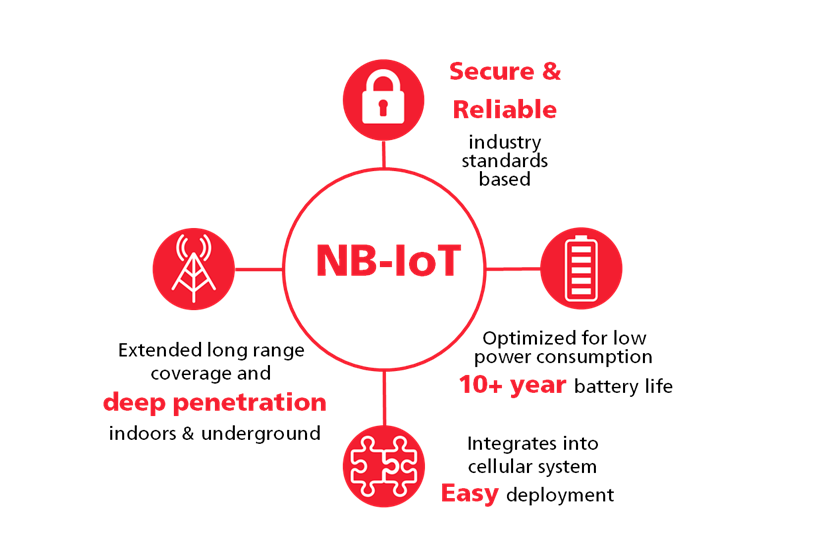
\includegraphics[width=0.98\textwidth]{pict/nb-iot.png}
    \caption{Features of NB-IoT \cite{ubox_nb-iot}}
    \label{fig:features_of_nb-iot}
\end{figure}

\subsection{LTE Cat-M}
LTE Cat-M, also known as eMTC, is a cellular LPWAN technology that was standardized by 3GPP in Release 13 in 2016. LTE Cat-M is an enhancement of LTE Cat-0, first introduced in release 12, that extends LTE with features improved to support Machine-Type Communications (MTC) and IoT. LTE Cat-M operates in the licensed spectrum, utilizing the already existing LTE resources \cite{icumt2019-lte-cat-m}, \cite{ubox_lte-cat-m}, \cite{Masek2021}.

LTE Cat-M supports two different data rates: 1 Mbps and 375 kbps. The maximum range of LTE Cat-M is 15 km in rural areas and 5 km in urban areas. LTE Cat-M uses power class 3 (23 dBm) and class 5 (20 dBm) defined by \href{https://www.3gpp.org/news-events/3gpp-news/nb-iot-complete}{3GPP}. LTE Cat-M uses a single antenna for downlink communication. LTE Cat-M supports both half-duplex and full-duplex communication \cite{icumt2019-lte-cat-m}, \cite{ubox_lte-cat-m}, \cite{Masek2021}. Key features of LTE Cat-M are depicted in Fig.\ref{fig:features-lte-m}.

\begin{figure}[h!]
    \centering
    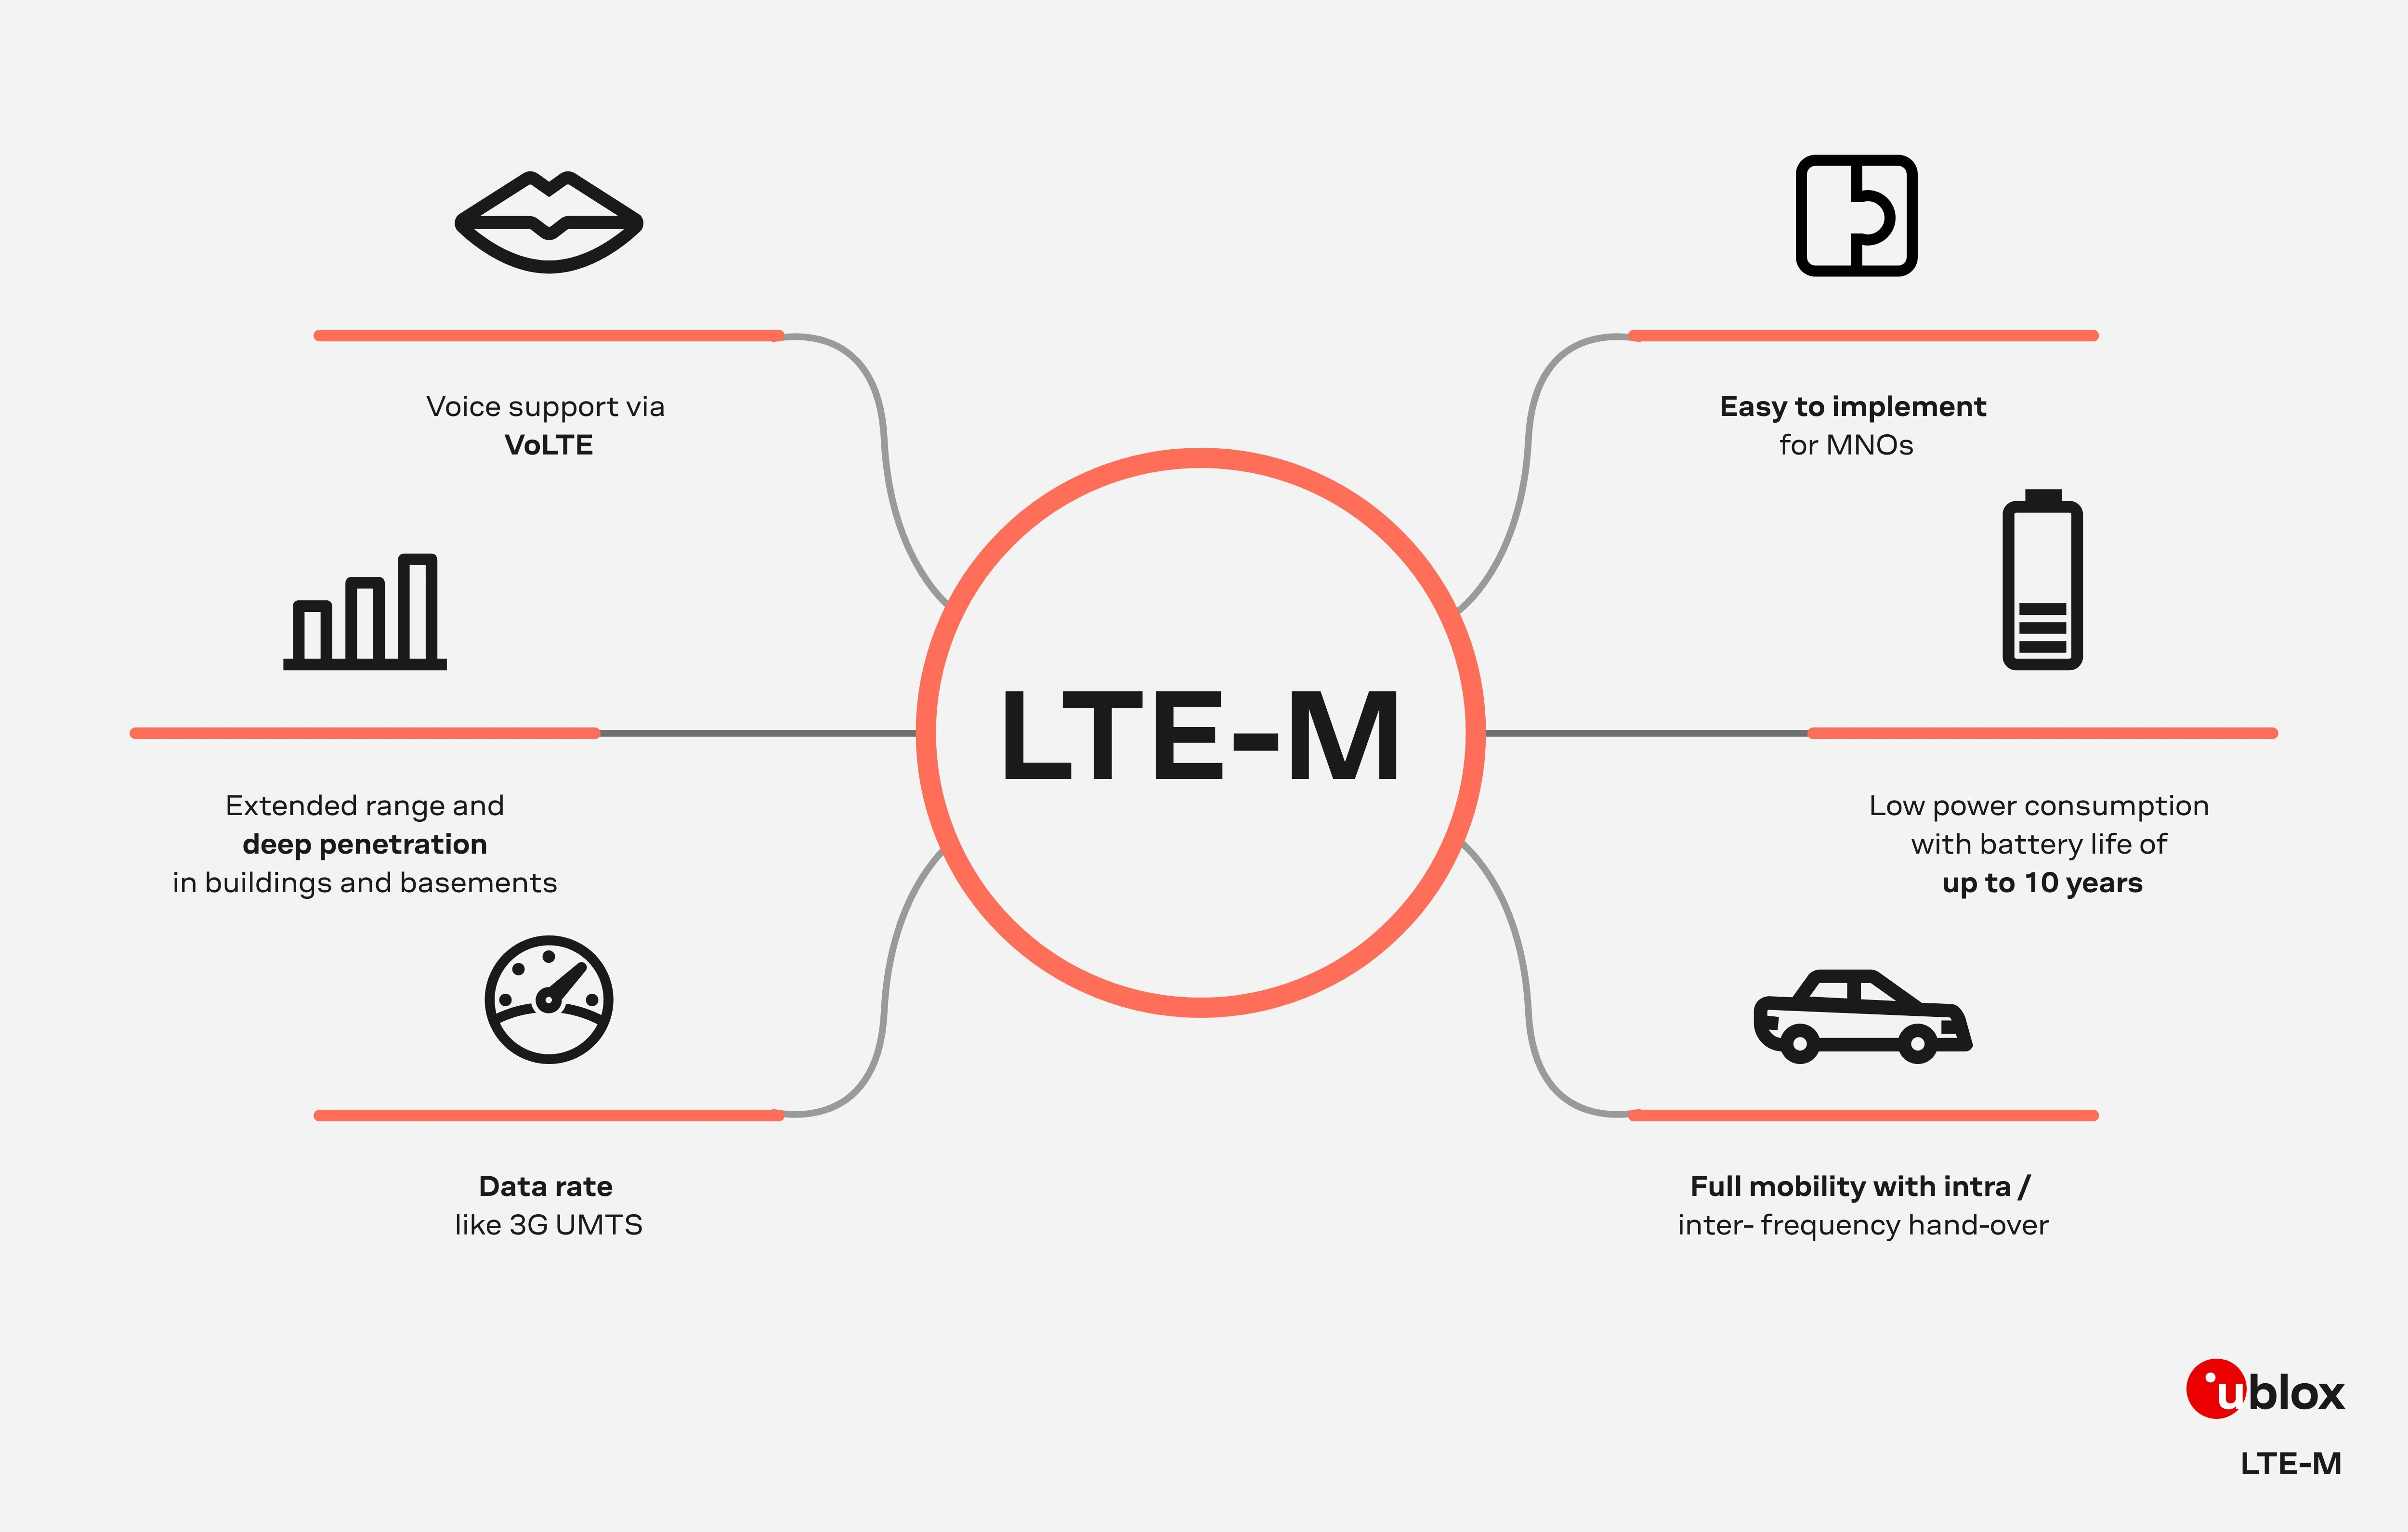
\includegraphics[width=\textwidth]{pict/lte-m-key-features.jpg}
    \caption{Key features of LTE CAT-M \cite{ubox_lte-cat-m}}
    \label{fig:features-lte-m}
\end{figure}

\subsection{LoRaWAN}
LoRaWAN is a non-cellular, open LPWAN technology protocol that is developed and maintained by the \href{https://lora-alliance.org/}{LoRa Aliiance}. The first specification was released in 2015. LoRaWAN operates in the unlicensed spectrum and can coexist with other unlicensed technologies such as Wi-Fi and Bluetooth. LoRaWAN supports two deployment modes: uplink-only and bidirectional. Uplink-only mode uses a single carrier frequency for both uplink and downlink communication, while bidirectional mode uses two carrier frequencies for uplink and downlink communication \cite{about-lorawan}, \cite{Mekki2018-overview-lpwan-tech} \cite{the-things-network}.

Data rates supported by LoRaWAN range between 300 bps and 50 kbps. The maximum range of LoRaWAN is 10 km in rural areas and 3 km in dense urban areas. LoRaWAN uses a single carrier frequency for both uplink and downlink communication. The uplink transmission power of LoRaWAN is 14 dBm, while the downlink transmission power is 20 dBm. LoRaWAN uses a single antenna for both uplink and downlink communication. LoRaWAN supports both half-duplex and full-duplex communication \cite{the-things-network}, \cite{about-lorawan}.

\subsection{Sigfox}
Sigfox is a non-cellular LPWAN technology that was developed by Sigfox in 2010, currently owned by \href{https://www.unabiz.com/iot-connectivity/#sigfox}{UnaBiz}. Sigfox operates in the unlicensed spectrum and can coexist with other unlicensed
technologies such as Wi-Fi and Bluetooth \cite{sigfox-start}. In Czech republic, Sigfox is maily operated by \href{http://sigfox.cz/cs}{SimpleCell}. Sigfox supports two deployment modes: uplink-only and bidirectional. Uplink-only mode uses a single carrier frequency for both uplink and downlink communication, while bidirectional mode uses two carrier frequencies for uplink and downlink communication \cite{Mekki2018-overview-lpwan-tech}.

Sigfox supports two different data rates: 100 bp and 600 bps. The average range of Sigfox is 40 km in rural areas and 10 km in urban areas. The transmission power in Europe is restricted to 14 dBm (25mW), with a duty cycle of only 1\%, and a transmission frequency of up to 140 mssages per day \cite{sigfox-start}  \cite{petrariu_sigfox-study}. 

The architecture of SigFox is depicted in Fig.\ref{fig:sigfox-archt}.

\begin{figure}[h!]
    \centering
    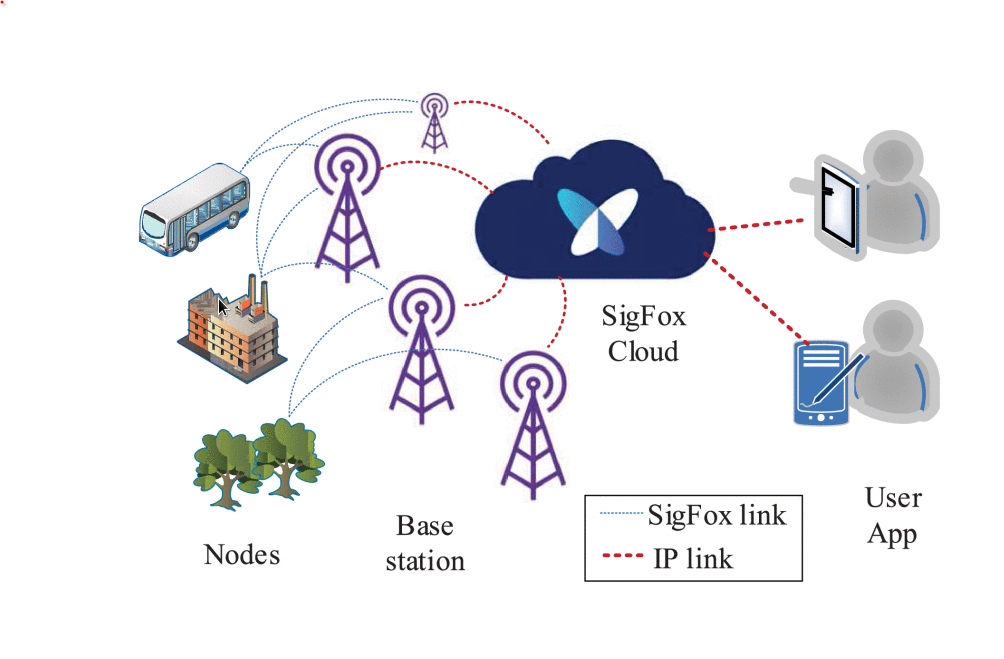
\includegraphics[width=0.98\textwidth]{pict/sigfox-archt.png}
    \caption{SigFox architecture \cite{petrariu_sigfox-study}}
    \label{fig:sigfox-archt}
\end{figure}


\subsection{Comparison of LPWAN Technologies}
The table in Fig.\ref{fig:compare-lpwan} compares the performance metrics of NB-IoT, Sigfox, LoRaWAN, and LTE Cat-M.

\iffalse
\begin{figure}[h!]
    \centering
    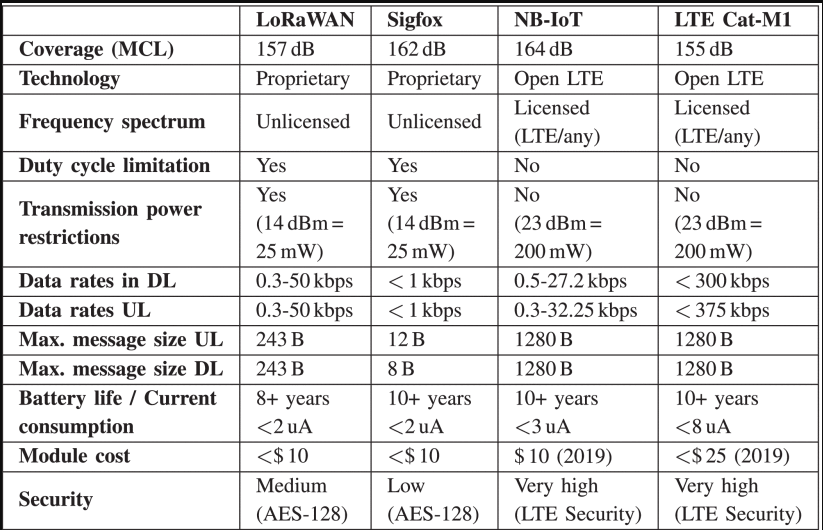
\includegraphics[width=\textwidth]{pict/compare-lpwan.png}
    \caption{Comparison of LPWAN Technologies \cite{icumt2019-lte-cat-m}}
    \label{fig:compare-lpwan}
\end{figure}
\fi

\begin{table}[ht]
\centering
\resizebox{\textwidth}{!}{%
\begin{tabular}{|l|c|c|c|c|}
\hline
\textbf{Parameter} & \textbf{LoRaWAN} & \textbf{Sigfox} & \textbf{NB-IoT} & \textbf{LTE Cat-M1} \\ \hline
    Coverage (MCL) & 157 dB & 162 dB & 164 dB & 155 dB \\ \hline
    Technology & Proprietary & Proprietary & Open LTE & Open LTE \\ \hline
    Frequency spectrum & Unlicensed & Unlicensed & Licensed (LTE/any) & Licensed (LTE/any) \\ \hline
    Duty cycle limitation & Yes & Yes & No & No \\ \hline
    Transmission power restrictions & 14 dBm (25 mW) & 14 dBm (25 mW) & 23 dBm (200 mW) & 23 dBm (200 mW) \\ \hline
    Data rates in DL & 0.3-50 kbps & < 1 kbps & 0.5-27.2 kbps & < 300 kbps \\ \hline
    Data rates UL & 0.3-50 kbps & < 1 kbps & 0.3-32.25 kbps & < 375 kbps \\ \hline
    Max. message size UL & 243 B & 12 B & 1280 B & 1280 B \\ \hline
    Max. message size DL & 243 B & 8 B & 1280 B & 1280 B \\ \hline
    Battery life / Current consumption & 8+ years <2 uA & 10+ years <2 uA & 10+ years <3 uA & 10+ years <8 uA \\ \hline
    Module cost & <$10 & <$10 & $10 (2019) & <$25 (2019) \\ \hline
    Security & Medium (AES-128) & Low (AES-128) & Very high (LTE Security) & Very high (LTE Security) \\ \hline
\end{tabular}%
}
\caption{Comparison of LoRaWAN, Sigfox, NB-IoT, and LTE Cat-M1}
\end{table}

\newpage
\section{Smart metering systems}











